% NICHT geeigent! deaktiviet die serielle Schnittstelle komplett!
% 5 Interfacing Options            Configure connections to peripherals
% P6 Serial                        Enable/Disable shell and kernel messages on the serial connection
% Would you like a login shell to be accessible over  serial? <No>
% The serial interface is disabled  <Ok>
%<Finish>
%Would you like to reboot now? <Ok>

%sudo systemctl disable serial-getty@ttyAMA0.service
%ps aux | grep getty

\textbf{Anschluss:} 

\begin{figure}[ht]
  \centering
  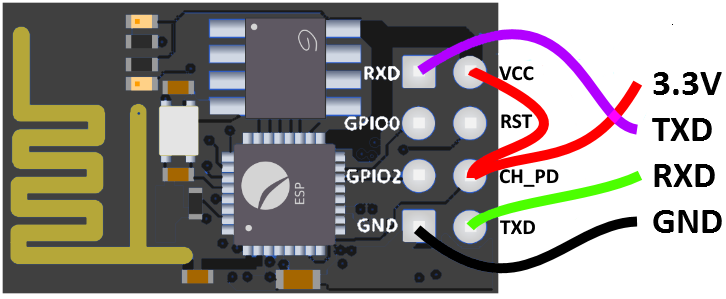
\includegraphics[scale=0.42]{images/ESP8266.png}	
  %	\caption{}
  \label{ESP8266-01}
\end{figure}


\begin{figure}[ht]
  \centering
  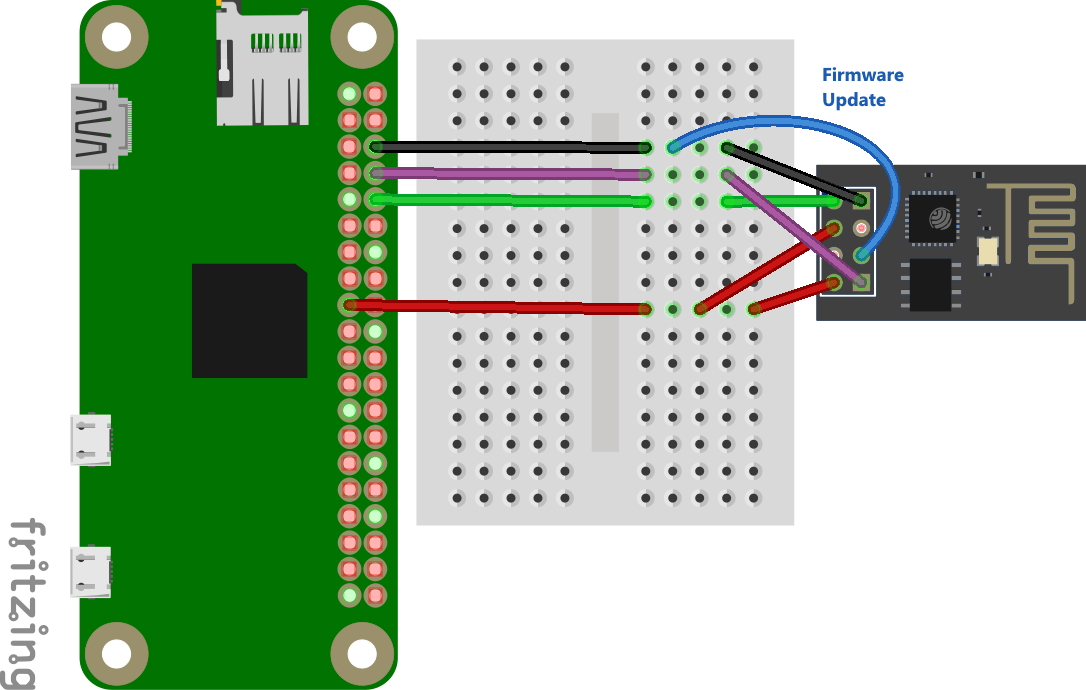
\includegraphics[scale=1.00]{images/ESP8266_ESP-01.png}	
  %	\caption{}
  \label{ESP8266_ESP-01}
\end{figure}


%\textbf{Firmware:}\\
%\url{http://www.electrodragon.com/w/ESP8266_AT-Command_firmware}

\textbf{AT-Befehlsatz:}\\
\url{https://www.itead.cc/wiki/images/5/53/Esp8266_at_instruction_set_en_v1.5.4_0.pdf}\\

\begin{figure}[ht]
  \centering
  
\includegraphics[scale=0.2]{images/QR_ESP8266_AT-Cmd.png}	
  %	\caption{}
  \label{ESP8266_AT-Cmd}
\end{figure}

 
\textbf{Raspberry Pi:}
\begin{console}
sudo systemctl stop serial-getty@ttyAMA0.service
sudo systemctl status serial-getty@ttyAMA0.service
sudo apt-get install minicom
sudo minicom -b 115200 -o -D /dev/ttyAMA0
\end{console}

\textbf{USB UART:} 
\begin{console}
sudo apt-get install minicom
sudo minicom -b 115200 -o -D /dev/ttyUSB0
\end{console}

Beispielkommunikation:

\begin{console}
Verbindungstest: AT<Enter><Strg>+j
\end{console}
\begin{screensmall}
OK
\end{screensmall}

\begin{console}
Reset: AT+RST<Enter><Strg>+j
\end{console}
\begin{screensmall}
 ets Jan  8 2013,rst cause:2, boot mode:(3,6)

load 0x40100000, len 1396, room 16
tail 4
chksum 0x89
load 0x3ffe8000, len 776, room 4
tail 4
chksum 0xe8
load 0x3ffe8308, len 540, room 4
tail 8
chksum 0xc0
csum 0xc0

2nd boot version : 1.4(b1)
  SPI Speed      : 40MHz
  SPI Mode       : DIO
  SPI Flash Size & Map: 8Mbit(512KB+512KB)
jump to run user1 @ 1000

Ai-Thinker Technology Co.,Ltd.

ready
\end{screensmall}

\begin{console}
Version abfragen: AT+GMR<Enter><Strg>+j
\end{console}

\begin{screensmall}
AT version:0.40.0.0(Aug  8 2015 14:45:58)
SDK version:1.3.0
Ai-Thinker Technology Co.,Ltd.
Build:1.3.0.2 Sep 11 2015 11:48:04
OK
\end{screensmall}

\begin{console}
WLAN Modus Station setzen: AT+CWMODE=1<Enter><Strg>+j
\end{console}

\begin{screensmall}
OK
\end{screensmall}

\begin{console}
Gefundene WLANs auflisten: AT+CWLAP<Enter><Strg>+j
\end{console}

\begin{screensmall}
+CWLAP:(3,"NETGEAR86",-86,"a0:63:91:ca:98:ca",6,-14)
+CWLAP:(4,"A1-PMC",-78,"a4:b1:e9:43:f4:d3",11,-41)
+CWLAP:(4,"Home",-92,"f4:06:8d:3b:e1:3c",11,-41)
+CWLAP:(3,"AndroidAP",-89,"10:a5:d0:73:de:eb",11,23)
\end{screensmall}

\begin{console}
Minicom beenden: <crtl><A><X>
\end{console}
